 \chapter{Caso 1: THREE.studies}

 THREE.studies es una pieza para el navegador que aprovecha las posibilildades del intercambio de flujos de audio y video. 

\section{Delimitacicón y contexto}

THREE.studies fue realizada en conjunto con Iracema de Andrade y con el apoyo técnico del colectivo PiranhaLab y fue apoyada por el programa Resiliencia Sonora de Música UNAM. El proyecto surge como un primer acercamiento a la realización de piezas que de alguna forma, puedan interactuar con intérpretes de forma remota. El contexto pandémico en este caso fue un detonador de una serie de pruebas realizadas para producir una pieza en tiempo real utilizando canales de comunicación en la web. 

SEALI 

\section{Versiones anteriores} 

La pieza fue estrenada en el marco del festival BEAST FEaST, organiado por la universidad de Birhminham. Cabe destascar que esta versión nunca tuvo una versión presencial. 

\begin{figure}[tb]
\centering
\subfloat[Primera Versión de THREE.studies]{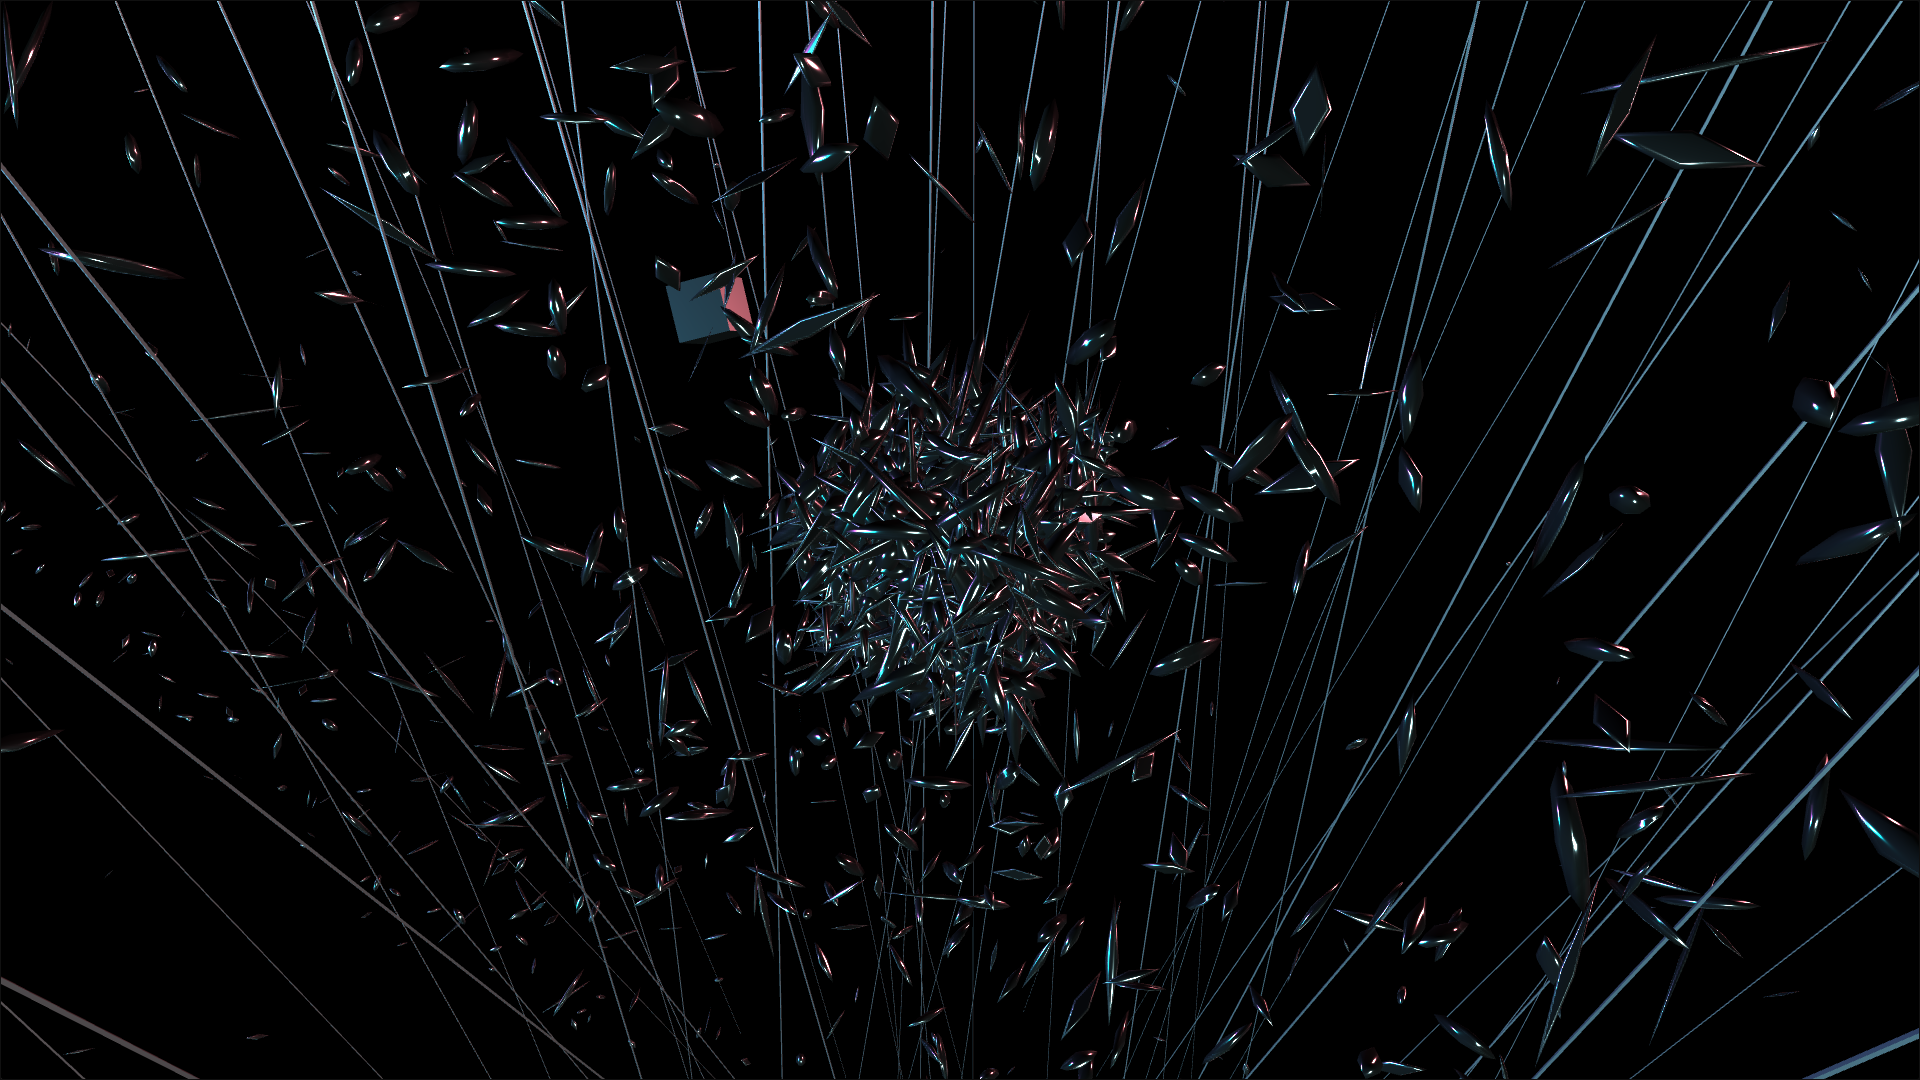
\includegraphics[width=\columnwidth]{../../img/beast.png}} \quad
\subfloat[Segunda versión de THREE.studies]{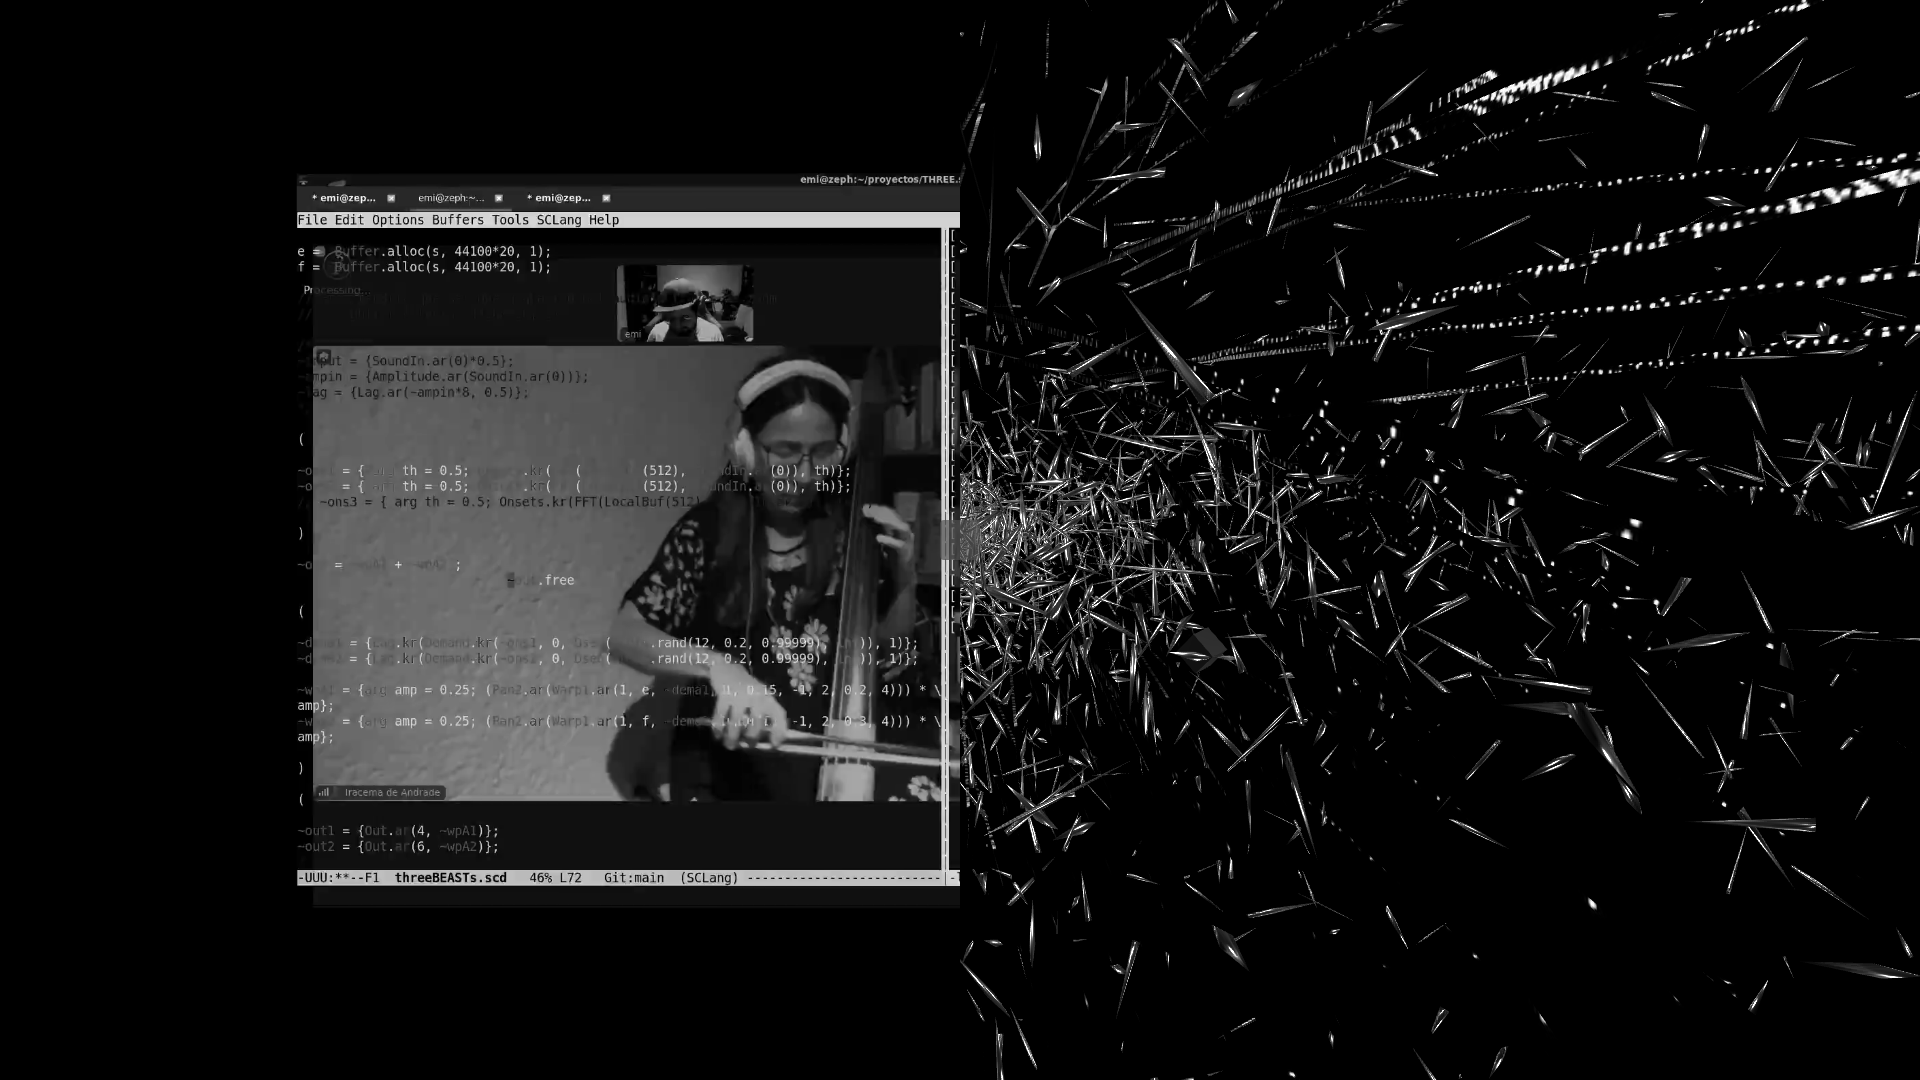
\includegraphics[width=\columnwidth]{../../img/threeNw.png}\label{fig:ipsum}} 
\caption[Versiones de THREE.studies]{Versiones de THREE.studies ordenadas cronológicamente} % The text in the square bracket is the caption for the list of figures while the text in the curly brackets is the figure caption
\label{fig:esempio}
\end{figure}

El proyecto se mantuvo en transformación. El video del proceso quedó registrado y fue posible utilizarlo para visualizarlo dentro del espacio virtual. 

\section{Version final}

El futuro podría implicar el uso de capturas tridimensionales de Iracema y reforzar el input de sonido a partir de la visualización de gestualidades fijadas en un objeto tridimensional. Una primera prueba del sistema basado en History podría implicar la reproducción del history como una pianola de código que pudiera imprimirse en el espacio virtual. En este sentido se podría prescindir de un video y dar cuenta del performance a partir de algunos efectos capturados del mismo: gestualidades en 3d, audio y código ejecutado en el tiempo. 
